\subsection{Problema a resolver}
El siguiente problema consiste en hallar un algoritmo capaz de dividir un conjunto de tareas ordenadas de forma tal que la realización de las mismas tenga costo total mínimo. El problema se ubica en una imprenta que cuenta con dos máquinas capaces de realizar distintas tareas de impresión. Estas máquinas deben ser preparadas de acuerdo al trabajo que vayan a realizar en ese momento. Dicha preparación requiere de un costo específico que depende del trabajo a realizar y del último ejecutado en esa máquina.\newline
\newline
Es importante considerar que los trabajos, $t_{1}$,...,$t_{n}$, pueden ser asignados a cualquiera de las dos máquinas, pero siempre respetando el orden en el que ingresan.\newline
\newline
Los datos otorgados consisten en los costos para preparar una máquina para el trabajo $t_{i}$ si antes se elaboró $t_{j}$, para cada par $t_{i}$ y $t_{j}$, con $j < i$. Por otro lado, se conoce el costo de preparar una máquina para cada trabajo al iniciar el día. Debe tenerse en cuenta que los costos son enteros positivos.\newline
\newline
El objetivo del problema consiste, entonces, en tomar la información de los trabajos a realizar y que el algoritmo generado sea capaz de indicar en qué máquina debe realizarse cada uno de ellos para que la suma de los costos de preparación de los mismos sea mínima.\newline
\newline
\textbf {Formatos de entrada y salida:}\newline
\newline
La entrada contiene varias instancias del problema. La primera línea de cada instancia contiene un entero positivo $n$ que indica la cantidad de trabajos ($t_{1},...,t_{n}$) a organizar. A esta línea le siguen $n$ líneas donde, en cada una de ellas, se indican los costos de preparación de cada trabajo. La $i$-ésima línea consta de los siguientes valores:

$$c_{0i}\ c_{1i}\ ...\ c_{(i-1)i}$$


donde \textbf{$c_{0i}$} es el costo de preparación de una máquina para $t_{i}$ si $t_{i}$ es el primer trabajo a realizar en esa máquina y $c_{ji}$ es el costo de preparación de una máquina para $t_{i}$ si $t_{j}$ es el último trabajo realizado en esa máquina. La entrada concluye con una línea comenzada por 0.\newline

La salida debe contener una línea por cada instancia de entrada, con el siguiente formato:

$$C\ k\ i_{1}\ ...\ i_{k}$$


donde \textbf{$C$} es el costo total de la solución, $k$ es la cantidad de trabajos asociados a una de las máquinas y los valores $i_{1},...,i_{k}$ son los índices de los trabajos asignados a esa máquina.\newline

En lo que sigue, presentaremos dos ejemplos del problema a resolver:
\begin{itemize}
\item {\large{\textbf{Ejemplo 1:}}}\newline
\newline
Para este ejemplo, decidimos elegir un posible caso del problema. En éste, pueden recorrerse los trabajos a realizar de forma ordenada hasta llegar a la solución óptima.\newline
\newline
\textbf{Formato de entrada:}
$$5$$
$$1$$
$$3\ \ 2$$
$$2\ \ 4\ \ 6$$
$$6\ \ 7\ \ 4\ \ 2$$
$$6\ \ 9\ \ 3\ \ 5\ \ 8$$

\begin{figure}[H] %[h] Aqui [b] para button [t] para top
\begin{center}
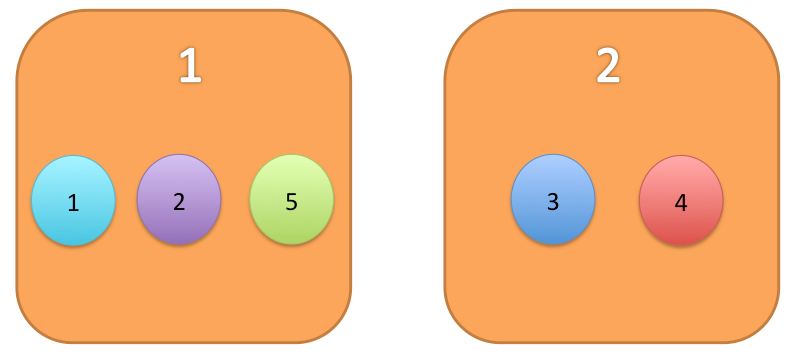
\includegraphics[width=250pt]{../imgs/ejemplo1ej1.jpg}
\caption{Ejemplo 1.}
\end{center}
\end{figure}

\textbf{Formato de salida:}
$$10\ \ 3\ \ 1\ \ 2\ \ 5$$
\item {\large{\textbf{Ejemplo 2:}}}\newline
\newline
En este caso, contrariamente al anterior, decidimos mostrar una situación en la que resultara extremadamente importante verificar todas las opciones posibles antes de tomar algún tipo de decisión sobre el armado de la solución al problema. En este caso, hasta no llegar al costo del último trabajo, cualquier decisión previa resulta inútil.\newline
\newline
\textbf{Formato de entrada:}
$$5$$
$$3$$
$$3\ \ 2$$
$$2\ \ 4\ \ 5$$
$$6\ \ 7\ \ 4\ \ 3$$
$$1\ \ 15\ \ 35\ \ 23\ \34$$

\begin{figure}[H] %[h] Aqui [b] para button [t] para top
\begin{center}
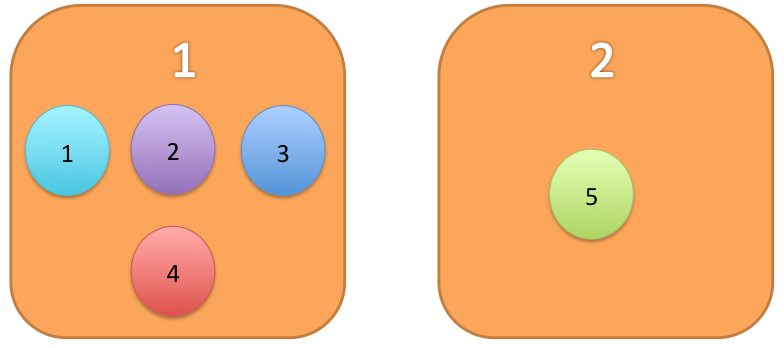
\includegraphics[width=250pt]{../imgs/ejemplo2ej1.jpg}
\caption{Ejemplo 2.}
\end{center}
\end{figure}

\textbf{Formato de salida:}
$$14\ \ 4\ \ 1\ \ 2\ \ 3\ \ 4$$
\end{itemize}

\subsection{Resolución coloquial}

Para resolver el problema descrito, consideramos armar todas las permutaciones posibles de los trabajos en las dos máquinas disponibles para realizarlos. Dado que contamos con dos máquinas y $n$ trabajos, las posibles combinaciones son $2^{n}$, siendo esta opción altamente costosa. Es entonces que decidimos resolver el problema utilizando $programación\ dinámica$.\newline
\newline
La $programación\ dinámica$, al igual que el método de Divide \& Conquer, resuelve problemas combinando las soluciones de sus subproblemas. A diferencia de este último, la $programación\ dinámica$ resuelve cada subproblema una única vez y almacena su solución en una tabla, evitando el trabajo de recomputar la respuesta cuando éste haya sido evaluado previamente.\newline
\newline
Luego, decidimos que nuestro programa almacenara las subsoluciones en una matriz del siguiente modo:
\begin{figure}[H]
\begin{center}
    \begin{tabular}{ l | l | l | l | l | l | l |}
    \multicolumn{7}{ |c| }{Máquina 1} \\
    \hline
    \multirow{5}{*}{\rotatebox{90}{\mbox{\centering{Máquina 2}}}} & \textbf{i/j} & \textbf{0} & \textbf{1} & ... & \textbf{(n-1)} & \textbf{n}\\ \cline{2-7}
    & \textbf{0} & $x_{00}$ & $x_{01}$ & ... & $x_{0(n-1)}$ & $x_{0n}$  \\ \cline{2-7}
   & \textbf{1} & $x_{10}$ & / & ... & $x_{1(n-1)}$ & $x_{1n}$ \\ \cline{2-7}
   & ... & ... & ... & ... & ... & ...\\ \cline{2-7}
   & \textbf{n} & $x_{n0}$ & $x_{n1}$ & ... & $x_{n(n-1)}$ & / \\ \cline{2-7}
    \end{tabular}
\caption{Matriz de almacenamiento de subproblemas calculados.}
\end{center}
\end{figure}
donde $x_{nm}$ representa el menor costo de realizar el trabajo $max(n,m)+1$ si la Máquina 1 realizó el trabajo $n$ y la 2 el $m$ previamente. Por otro lado, '/' representa que dicha casilla no puede ser completada dado que $i = j$, y un mismo trabajo no puede haberse realizado en ambas máquinas en una ejecución. El valor 0 representa el estado inicial de cada máquina.\newline
\newline
Por lo tanto, los casos que contempla nuestro algoritmo son de la siguiente forma:
\begin{figure}[H] %[h] Aqui [b] para button [t] para top
\begin{center}
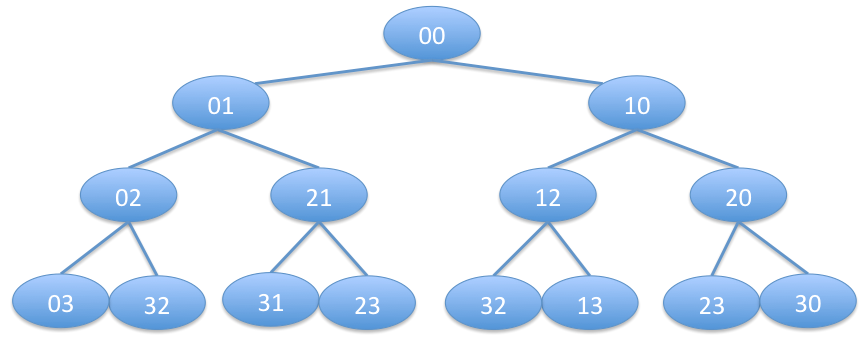
\includegraphics[width=400pt]{../imgs/arbol.jpg}
\caption{Árbol de decisiones del modelado del problema.}{\textit{Prueba con cantidad de trabajos = 3.}}
\end{center}
\end{figure}
Donde en cada \raisebox{-.1\height}{
\includegraphics[width=40pt]{../imgs/leyendaArbol.jpg}}, $m$ representa al último trabajo realizado en la máquina 1 y $n$ al realizado en la máquina 2. El estado \raisebox{-.1\height}{
\includegraphics[width=40pt]{../imgs/Cerocero.jpg}} representa el estado inicial del problema, en el que no hay trabajos. Como puede observarse, se repiten una gran cantidad de casos dado que las máquinas son indistinguibles entre sí, luego \raisebox{-.1\height}{
\includegraphics[width=40pt]{../imgs/ij.jpg}}=\raisebox{-.1\height}{
\includegraphics[width=40pt]{../imgs/ji.jpg}} para cada $i \neq j$. Por lo tanto, recalcular los costos resulta, además de altamente costoso, innecesario, siendo la $programación\ dinámica$ un método adecuado para la realización del algoritmo.

El pseudocódigo que resuelve el problema es el siguiente:\newline
\newline
%no se hacer pseudo sobre matrices jijiji
\begin{algorithm}[H]
    \SetAlgoLined
    \caption{MinimizacióndeCostosdeTareas}
    \KwIn{Entero $m1$, Entero $m2$, Entero $cantidadDeTrabajos$, Costos $cs$, Matriz $valores$}
    \KwOut{Costo $c$}
    
    Entero $siguienteTrabajo$ = $max(m1,m2)+1$\\ 
    \If{$siguienteTrabajo > cantidadDeTrabajos$}{
        $c$ = 0
    }\\
    \eIf{$valores[m1][m2]>-1$}{
        $c$ = $valores[m1][m2]$
    }{
        Entero $costo1$ = cs[siguienteTrabajo-1][m1] +\\ MinimizacióndeCostosdeTareas(siguienteTrabajo,m2)\\
        Entero $costo2$ = cs[siguienteTrabajo-1][m2] +\\ MinimizacióndeCostosdeTareas(m1, siguienteTrabajo)\\
        \eIf{$costo1 < costo2$}{
            $valores[m1][m2] = costo1$\\
            $valores[m2][m1] = costo1$\\        
            $c$ = $costo1$\\
        }{
            $valores[m1][m2] = costo2$\\
            $valores[m2][m1] = costo2$\\        
            $c$ = $costo2$\\
        }
    }\\
    \textbf{devolver} $c$
\end{algorithm}

\begin{algorithm}[H]
    \SetAlgoLined
    \caption{inicializarMinimizacionDeCostos}
    \KwIn{Entero $cantidadDeTrabajos$}
    \KwOut{Costo $c$, Entero $cantidadAsociada$, $listaIndices$}



    \lIf{$cs = \emptyset$}{\textbf{devolver} 0, 0, $ListaVacia$}\\
    Entero $costoMinimo$ = MinimizacióndeCostosdeTareas(0,0)\\

    Lista $maquina1$\\

    \For{Entero i=1 a $cantidadDeTrabajos$}{
        \eIf{$valores[i][m2] < valores[m1][i]$}{
            $m1 = i$\\
        }{
            $m2 = i$\\
            $maquina1$ \leftarrow i\\
        }
    }

    \textbf{devolver} $costoMinimo, |maquina1|, maquina1$\\

    
\end{algorithm} 

Donde $Costos$ es una matriz que contiene los costos de poner un trabajo $i$ en una máquina si previamente se realizó el trabajo $j$ en ella misma, con $j<i$. Por otro lado, $maquina1$ consiste en una lista de los trabajos que realiza la máquina a la que se le inserta el primer trabajo.

\newpage
\subsection{Demostración de correctitud}

Veamos que el algoritmo realizado es correcto. Empecemos por demostrar que cada subproblema es óptimo. Para ello, consideremos que cada uno de éstos consiste en determinar en qué máquina debe ubicarse el trabajo $x$ si en la 1 se encuentra el $i$ y en la 2 el $j$, con $x=max(i,j)+1$, tal que el costo sea mínimo. Esto significa que, dadas dos opciones posibles, nuestro algoritmo calcula ambas y selecciona la de menor costo en cada subproblema. De este modo, nuestro algoritmo recorre todas las secuencias de decisiones almacenando las subsoluciones óptimas.

Luego, demostremos que nuestro algoritmo cumple con el Principio de optimalidad de Bellman para corroborar su correctitud.\footnote{Dada una secuencia óptima de decisiones, toda subsecuencia de ella es, a su vez, óptima.} Para ello, supongamos que éste devuelve la solución óptima $S$. Dicha solución se encuentra conformada por todas subsoluciones óptimas salvo una, $x_{i}$. Luego, reemplacemos $x_{i}$ por la solución óptima de su subproblema correspondiente\footnote{Sabemos que existe una subsolución óptima pues estamos ante un conjunto no vacío de soluciones y todo conjunto acotado no vacío alcanza un mínimo local.}, llamemos $S^*$ a esta nueva solución. Pero entonces, $S^*$ tiene un costo final menor que $S$. Esto resulta absurdo pues supusimos que $S$ era solución óptima. Luego, todas las subsoluciones de $S$ son óptimas implicando que la solución final también lo es. Entonces, queda demostrado que nuestro algoritmo cumple con el Principio de optimalidad de Bellman confirmando su optimalidad.

% demostrar usando http://webdiis.unizar.es/asignaturas/EDA/ea/slides/4-Programacion%20dinamica.pdf
\subsection{Complejidad del algoritmo}

Veamos que nuestro agoritmo cumple con la complejidad requerida. Para ello, llamemos $n$ a la cantidad total de trabajos a realizar:
\begin{itemize}
\item En primer lugar, la función \textbf{inicializarMinimizacionDeCostos} inicializa la matriz $valores$ con una dimensión de $n^*n$ y aplica una única vez la función \textbf{resize} ($\mathcal{O}(n)$)\footnote{http://en.cppreference.com/w/cpp/container/vector/resize}. Dicha matriz se encuentra representada por un vector de vectores cuyo espacio de memoria es reservado para que las asignaciones se realicen en $\mathcal{O}(1)$. Dado que la función la recorre una única vez para inicializarla, el costo temporal resulta $\mathcal{O}(n^{2})$. Por otro lado, se utilizan las funciones $size()$($\mathcal{O}(1)$)\footnote{http://en.cppreference.com/w/cpp/container/vector/size} y $push\_back()$($\mathcal{O}(1)$)\footnote{http://en.cppreference.com/w/cpp/container/vector/push\_back} pero, dado que sus complejidades no resultan significativas frente a la complejidad final de la función, no son consideradas para el cálculo de la misma. Luego, la complejidad de \textbf{inicializarMinimizacionDeCostos} resulta $\mathcal{O}(n^{2})$.

\item Por otro lado, se realiza un llamado a \textbf{MinimizacióndeCostosdeTareas}. Veamos que una vez completada la matriz $valores$, la complejidad de la función recursiva se torna constante y puede verse acotada por el tamaño de la matriz ($n^{2}$).
\begin{itemize}
\item En cada llamada recursiva a \textbf{MinimizacióndeCostosdeTareas}, se determina en qué máquina se ubica el $sigTrabajo$. Para tomar dicha decisión, se realizan operaciones de tiempo lineal y se ejecuta recursivamente la función dos veces. En la primera, agregando el trabajo en la máquina 1 y, en la segunda, agregando el trabajo en la máquina 2. De esta manera, se calculan las soluciones a dichos subproblemas a menos que los resultados de éstos ya se encuentren en la matriz $valores$ (dado que ésta abarca todas las subsoluciones posibles), acotando dicha ejecución por $\mathcal{O}(n^{2})$. A partir de esto, podemos determinar que el peor caso consiste en llenar la matriz entera ($\mathcal{O}(n^{2})$) y que las soluciones a las llamadas recursivas siguientes se encuentren en ella, tornándolas constantes. Por lo tanto, el costo temporal de la llamada recursiva se encuentra acotado por la matriz, luego, por $\mathcal{O}(n^{2})$. 

\item Una vez almacenadas todas las subsoluciones en $valores$, se procede armando la solución final. Para ello, se reproducen las decisiones tomadas en cada paso a partir de la matriz. Dicho procedimiento se ejecuta en \textbf{inicializarMinimizacionDeCostos}, con un ciclo de 1 hasta $n$ que compara, en cada paso, dos valores enteros de la matriz. Luego, este extracto tiene una complejidad de $\mathcal{O}(n)$ ya que las comparaciones se realizan en $\mathcal{O}(1)$.

\end{itemize}
\item Por lo tanto, el costo temporal de \textbf{inicializarMinimizacionDeCostos} es $\mathcal{O}(n^{2})$ y el de \textbf{MinimizaciondeCostosdeTareas} es $\mathcal{O}(n^{2})$ y, dado que dichas funciones se realizan en forma paralela, la complejidad temporal final es $\mathcal{O}(2n^{2})$, que se encuentra acotado por $\mathcal{O}(n^{2})$. 
\end{itemize}

\subsection{Instancias posibles}
Para verificar la correctitud de nuestro programa, dispusimos variar estratégicamente las instancias de entrada al ejecutarlo.
\begin{itemize}
\item En primer lugar, ejecutamos el programa ingresando trabajos de igual costo independientemente del trabajo realizado anteriormente. De este modo, verificamos que nuestro algoritmo organizara los trabajos tal como esperado cuando más de una combinación posible fuera solución.\newline

\textbf{Parámetro de entrada:} $$5$$
$$5$$
$$5\ \ 5$$
$$5\ \ 5\ \ 5$$
$$5\ \ 5\ \ 5\ \ 5$$
$$5\ \ 5\ \ 5\ \ 5\ \ 5$$
\textbf{Parámetro de salida:} $$25\ \ 4\ \ 1\ \ 2\ \ 3\ \ 4$$\\
\item Por otra parte, probamos no ingresar ningún trabajo para corroborar que la salida estuviera comprendida por un costo 0, una cantidad de trabajos asociados a una máquina igual a 0 y una lista vacía.\newline

\textbf{Parámetro de entrada:} $$0$$
\textbf{Parámetro de salida:} $$0\ \ 0 \ \ 0$$

\item Luego, probamos ingresar costos que implicaran que todos los trabajos debían realizarse en una misma máquina con el fin de verificar que esto, efectivamente, ocurriera.\newline

\textbf{Parámetro de entrada:} $$5$$
$$4$$
$$7\ \ 4$$
$$8\ \ 9\ \ 5$$
$$6\ \ 7\ \ 5\ \ 2$$
$$5\ \ 6\ \ 8\ \ 9\ \ 1$$
\textbf{Parámetro de salida:} $$16\ \ 5 \ \ 1\ \ 2\ \ 3\ \ 4\ \ 5$$
\end{itemize}

De este modo, logramos abarcar los casos límite en los que la implementación pudiera haber encontrado algún problema. Dado que los resultados obtenidos fueron los esperados, determinamos que para todas las instancias válidas posibles de entrada nuestra implementación resulta correcta.

\subsection{Experimentación}
Para las pruebas de complejidad empírica, generamos instancias aleatorias de costos de los trabajos alterando la cantidad de los mismos. Estas instancias fueron generadas en $C++$ con la función $rand()$. La cantidad de trabajos generados se comprendió entre 100 y 32300, agregando de a 100 en cada iteración. Las mediciones de tiempo en nanosegundos se realizaron con la función $high\ resolution\ clock$\footnote{http://en.cppreference.com/w/cpp/chrono/high\_resolution\_clock} de la librería $Chrono$ de $C++$. Debido a que éstas fueron realizadas en nanosegundos, las pruebas cuyo tamaño de entrada era menor a 1000 se realizaban en mayor tiempo que las instancias más grandes pues el procesador les otorgaba menos atención al realizar cambio de contexto. De este modo, logramos medir las pruebas de nuestro algoritmo para comprobar que la complejidad correspondiera con la mencionada anteriormente.

Las funciones de complejidad con las que se compararon nuestros gráficos de tiempo fueron ajustadas por algoritmos matemáticos (proporcionados por \textbf{sci davis}). Dichos algoritmos se encargaron de multiplicarle y sumarle constantes a las funciones con el fin de que éstas se ajustaran a nuestros resultados sin modificar el comportamiento de las funciones utilizadas para comparar.

\begin{figure}[H] %[h] Aqui [b] para button [t] para top
\begin{center}
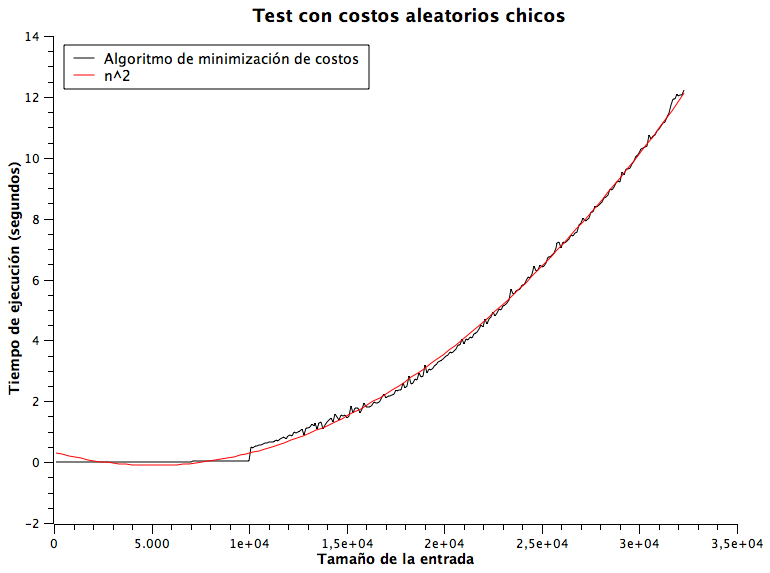
\includegraphics[width=350pt]{../tests/ej1/testChico.png}
\end{center}
\end{figure}
En este caso, utilizamos instancias de números aleatorios entre 1 y 150. En este gráfico, se puede ver de forma clara que la función de la complejidad se adapta perfectamente a los datos obtenidos. De este modo, se deja en evidencia la complejidad esperada.


La función utilizada para aproximar nuestros valores resultantes luego de las distintas ejecuciones fue $a_{0} + a_{1}x + a_{2}x^{2}$.
En este caso, los valores que aproximan la función a nuestros datos son:
$$desde\ x = 100\ a\ x = 32.300$$
$$a_{0} = 0,32423419158503$$
$$a_{1} = -0,00016812837387441$$
$$a_{2} = 1,65040451628269e^{-8}$$

% ---------------------------------------------------------------------------------------
% Polynomial fit of dataset: Table1_2, using function: a0+a1*x+a2*x^2
% Y standard errors: Unknown
% From x = 100 to x = 32.300
% a0  = 0,32423419158503 +/- 0,0215946299831477
% a1  = -0,00016812837387441 +/- 3,07784412487107e-06
% a2  = 1,65040451628269e-08 +/- 9,19965264096027e-11
% --------------------------------------------------------------------------------------
% Chi^2/doF = 0,0165295926762495
% R^2 = 0,998773136476792
% ---------------------------------------------------------------------------------------

\begin{figure}[H] %[h] Aqui [b] para button [t] para top
\begin{center}
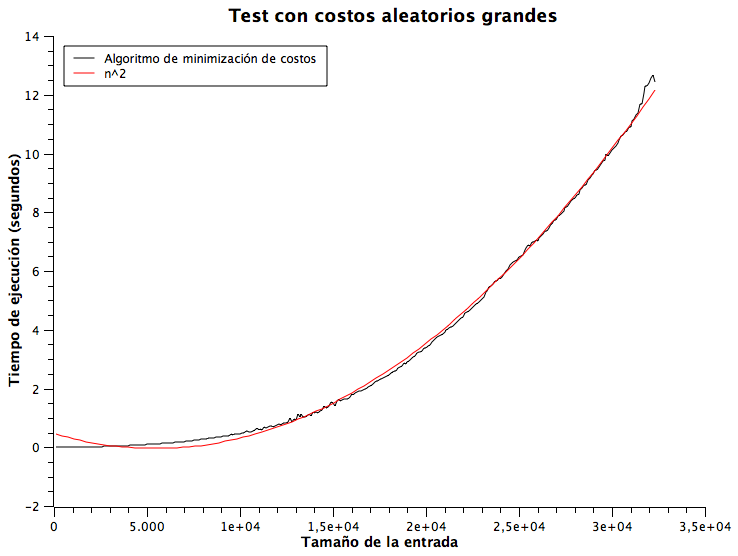
\includegraphics[width=350pt]{../tests/ej1/testGrande.png}
\end{center}
\end{figure}

En este caso, utilizamos instancias de números aleatorios entre 500 y 1500. Al igual que en la situación anterior, se puede observar que la función de complejidad se acerca perfectamente a los valores devueltos por las distintas ejecuciones del programa. En esta situación, encontramos que la magnitud de los costos de los trabajos no afectan la complejidad, y esto tiene sentido ya que la complejidad se encuentra determinada por la cantidad de trabajos ingresados.

La función utilizada para aproximar nuestros valores resultantes luego de las distintas ejecuciones fue $a_{0} + a_{1}x + a_{2}x^{2}$.
En este caso, los valores que aproximan la función a nuestros datos son:

$$desde\ x = 100\ a\ x = 32.300$$
$$a_{0}  = 0,463420767939423$$
$$a_{1}  = -0,000185064576979962$$
$$a_{2}  = 1,69442722903951e^{-8}$$

% ---------------------------------------------------------------------------------------
% [29/09/13 15:11 Plot: ''Graph1'']
% Polynomial fit of dataset: Table1_2, using function: a0+a1*x+a2*x^2
% Y standard errors: Unknown
% From x = 100 to x = 32.300
% a0  = 0,463420767939423 +/- 0,0259887707740958
% a1  = -0,000185064576979962 +/- 3,70188804599674e-06
% a2  = 1,69442722903951e-08 +/- 1,10661696857655e-10
% --------------------------------------------------------------------------------------
% Chi^2/doF = 0,0239117967063003
% R^2 = 0,998216395272766
% ---------------------------------------------------------------------------------------

\begin{figure}[H] %[h] Aqui [b] para button [t] para top
\begin{center}
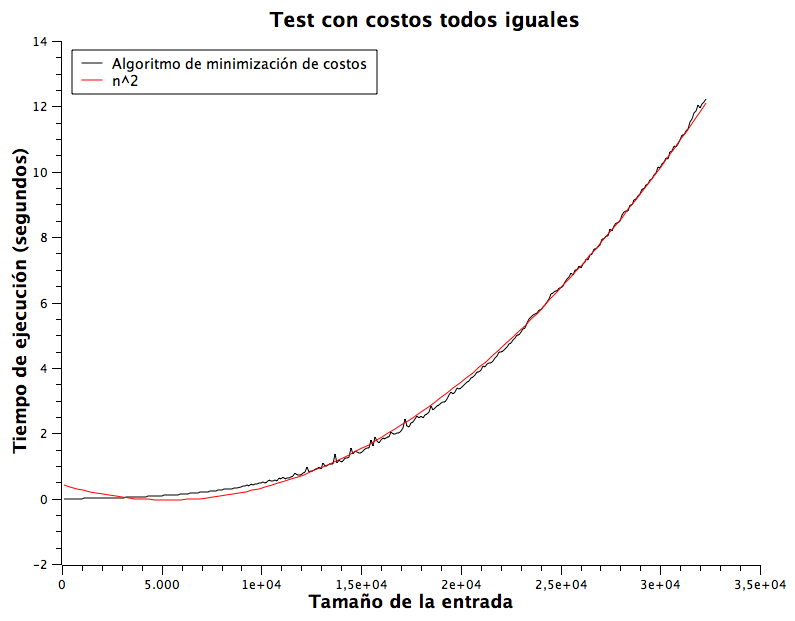
\includegraphics[width=350pt]{../tests/ej1/testIguales.png}
\end{center}
\end{figure}

En este caso, utilizamos instancias cuyos valores son todos iguales. Esto implica que existen múltiples soluciones al problema, y que el programa debe contemplar cada una de ellas. Al observar los resultados, llegamos a la conclusión de que la cantidad de soluciones posibles no es un factor significante a la hora de medir la complejidad de las ejecuciones. Esto se debe a que, a pesar de encontrar una solución al problema, el algoritmo debe probar con todas las demás posibilidades para comprobar que no exista una mejor.

La función utilizada para aproximar nuestros valores resultantes luego de las distintas ejecuciones fue $a_{0} + a_{1}x + a_{2}x^{2}$.
En este caso, los valores que aproximan la función a nuestros datos son:

$$desde\ x = 100\ a\ x = 32.300$$
$$a_{0}  = 0,424466923410826$$
$$a_{1}  = -0,000176224064649403$$
$$a_{2}  = 1,66520770037108e^{-8}$$


% ---------------------------------------------------------------------------------------
% [29/09/13 15:27 Plot: ''Graph1'']
% Polynomial fit of dataset: Table1_2, using function: a0+a1*x+a2*x^2
% Y standard errors: Unknown
% From x = 100 to x = 32.300
% a0  = 0,424466923410826 +/- 0,0221964720229293
% a1  = -0,000176224064649403 +/- 3,16061236730305e-06
% a2  = 1,66520770037108e-08 +/- 9,44987080940012e-11
% --------------------------------------------------------------------------------------
% Chi^2/doF = 0,0174278400512325
% R^2 = 0,998690483561816
% ---------------------------------------------------------------------------------------


